\section{Rund um das LVS}

Alle modernen Geräte verfügen über 3 Antennen.

Es sendet jeweils nur eine Antenne.

Im Suchmodus empfangen alle Antennen.

\begin{center}
  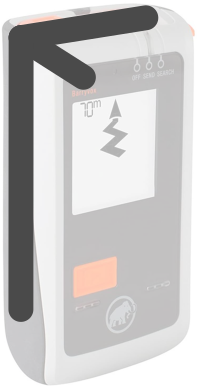
\includegraphics[width=0.65\linewidth]{antennas.svg.pdf}
\end{center}

Die Antennen sind empfindlich gegen Erschütterungen, es ist also behutsam mit dem LVS umzugehen um den Bruch einer oder mehrerer Antennen zu vermeiden.

\newcolumn

Elektronische Geräte und metallische Gegenstände stören das LVS bei der Arbeit, darum gilt:

\begin{itemize}
  \item{Im Sendemodus mindestens 20 cm Abstand}
  \item{Im Suchmodus mindestens 50 cm Abstand}
  \item{Während einer Verschüttetensuche mindestens 10 m Abstand zu Mobiltelefone und Funkgeräte im aktiven Betrieb (Funken bzw. Telefonieren)}
\end{itemize}

\textit{Die modernen LVS weisen im Suchmodus auch akustisch und/oder visuell auf eine vorhandene Störquelle hin.}

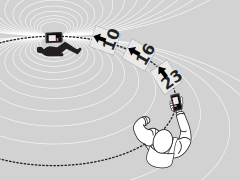
\includegraphics[width=\linewidth]{lvs-search.svg.pdf}

Das Gerät leitet die Suche entlang der Feldlinien: \textit{Es ist also völlig normal bei der Suche eine Kurve zu beschreiten.}

Die effektive Reichweite eines LVS ist Geräteabhängig. In der Praxis hat sich eine Suchstreifenbreite von ca. 40 m bewährt. Also vom Gerät ausgehend 20 m in jede Richtung.

Die Distanzangabe auf dem Gerät entspricht in etwa der Kurvenlänge auf der Feldlinie.

\newcolumn

Um die Suchrichtung festzustellen muss das Gerät in Bewegung sein: \textit{Ich kann also nicht an einem Ort stehen bleiben um die Suchrichtung zu bestimmen.}

Die Suche mit dem LVS unterteilt sich in 4 Phasen:

\begin{enumerate}
  \item{
    \textbf{Signalsuche} -- solange kein Signal empfangen
    \begin{itemize}
      \item{Suche nach optischen Hinweisen}
      \item{Suche nach akustischen Hinweisen}
      \item{Suche nach erstem Signal mit dem LVS}
    \end{itemize}
  }
  \item{
    \textbf{Grobsuche} -- bis auf 3 m 
    \begin{itemize}
      \item{Der Richtungsangabe auf dem LVS folgen}
      \item{Ruckartige Bewegungen vermeiden}
    \end{itemize}
  }
  \item{
    \textbf{Feinsuche} -- bis Minimaldistanz
    \begin{itemize}
      \item{Suche etwa auf Kniehöhe}
      \item{LVS nicht mehr neu ausrichten}
      \item{Suche nach Minimaldistanz}
    \end{itemize}
  }
  \item{
    \textbf{Punktsuche} -- bis Treffer mit der Sonde
    \begin{itemize}
      \item{Sondieren, ausgehend von Minimaldistanz}
      \item{Bei Treffer Sonde stecken lassen}
      \item{Umgehend mit der Bergung beginnen}
    \end{itemize}
  }
\end{enumerate}

Es gilt schnellstmöglich Kopf und Brustkorb des Lawinenopfers freizulegen.
Ohne Lebenszeichen sofort mit der Reanimation beginnen.

Ist das Lawinenopfer bei vollem Bewusstsein, soll das Wiederaufwärmen durch aktive Bewegung und warme Getränke erfolgen.
Bei Bewusstseinstrübung oder Ohnmacht sollten weitere Bewegungen allerdings vermieden werden: Stattdessen vor weiterem Auskühlen schützen und nach Möglichkeit warme Getränke verabreichen.

\textbf{Bei einem Lawinenunfall sind die ersten 15 Minuten entscheidend, danach sinkt die Überlebenschance deutlich.}

\newcolumn

Es wird empfohlen das LVS mit dem dazugehörigen Gurtsystem zu tragen.
Dabei sollte das LVS immer von mindestens einer Schicht Kleidung bedeckt sein.

\begin{center}
  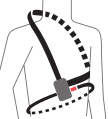
\includegraphics[width=0.48\linewidth]{lvs-harness.svg.pdf}
  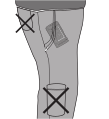
\includegraphics[width=0.48\linewidth]{lvs-pocket.svg.pdf}
\end{center}

Alternativ kann das LVS auch in einer Hosentasche mitgeführt werden.
Für die Hosentasche gilt dabei:

\begin{itemize}
  \item{Sie muss über einen Reissverschluss verfügen.}
  \item{Sie darf nicht auf die Hose aufgenäht sein.}
  \item{Gesässtaschen sind nicht geeignet.}
\end{itemize}

Das LVS sollte am Anfang der Saison mit frischen Batterien bestückt werden.
Damit die Batterien nicht auslaufen und das Gerät beschädigen können sollten diese am Ende der Saison herausgenommen werden.
\textbf{Keine wiederaufladbaren Batterien verwenden.}

Die genaue Laufzeit ist abhängig vom Gerät, beträgt im Sendemodus aber in etwa 200 Stunden.
Im Suchmodus hingegen nur 1 Stunde.

\textbf{Das LVS muss während der gesamten Tour im Sendemodus eingeschaltet sein.}
Ausschalten auf dem Gipfel oder während einer Pause zum Batterien sparen ist nicht notwendig.

\newcolumn
